\documentclass[hidelinks,11pt,dvipsnames]{article}
% xcolor commonly causes option clashes, this fixes that
\PassOptionsToPackage{dvipsnames,table}{xcolor}
\usepackage[tmargin=1in, bmargin=1in, lmargin=0.8in, rmargin=1in]{geometry}

%%%%%%%%%%%%%%%%%%%%%%%%%%%%%%%%%%%%%%%%%%%%%%%%%%%%%%%%%%%%%%%%%%%%
%%% For inkscape-figures
%%% Assumes the following directory structure:
%%% master.tex
%%% figures/
%%%     figure1.pdf_tex
%%%     figure1.svg
%%%     figure1.pdf
%%%%%%%%%%%%%%%%%%%%%%%%%%%%%%%%%%%%%%%%%%%%%%%%%%%%%%%%%%%%%%%%%%%%
%\usepackage{import}
\usepackage{pdfpages}
\usepackage{transparent}

\newcommand{\incfig}[2][1]{%
    \def\svgwidth{#1\columnwidth}
    \import{./figures/}{#2.pdf_tex}
}

\pdfsuppresswarningpagegroup=1

% enable synctex for inverse search, whatever synctex is
\synctex=1
\usepackage{float,macrosabound,homework,theorem-env}
\usepackage{microtype}


% font stuff
\usepackage{sectsty}
\allsectionsfont{\sffamily}
\linespread{1.1}

% bibtex stuff
\usepackage[backend=biber,style=alphabetic,sorting=anyt]{biblatex}
\addbibresource{main.bib}

% colored text shortcuts
\newcommand{\blue}[1]{\color{MidnightBlue}{#1}}
\newcommand{\red}[1]{\textcolor{Mahogany}{#1}}
\newcommand{\green}[1]{\textcolor{ForestGreen}{#1}}


% use mathptmx pkg while using default mathcal font
\DeclareMathAlphabet{\mathcal}{OMS}{cmsy}{m}{n}

% fixes the positioning of subscripts in $$ $$
\renewcommand{\det}{\operatorname{det}}

\usetikzlibrary{positioning, arrows.meta}
\newcommand{\here}[2]{\tikz[remember picture]{\node[inner sep=0](#2){#1}}}

%%%%%%%%%%%%%%%%%%%%%%%%%%%%%%%%%%%%%%%%%%%%%%%%%%%%%%%%%%%%%%%%%%%%%
%%% Entry Counter
%%%%%%%%%%%%%%%%%%%%%%%%%%%%%%%%%%%%%%%%%%%%%%%%%%%%%%%%%%%%%%%%%%%%%
\newcounter{entry-counter}
\newcommand{\entry}[1]
{
	\addtocounter{entry-counter}{1}
    \tchap{Entry \arabic{entry-counter}}
	%\addcontentsline{toc}{section}{Entry \arabic{entry-counter}: #1}
	\vspace{-1.5em}
    \begin{center}
		\small \emph{Written: #1}
    \end{center}
}

\usepackage{titling}
\renewcommand\maketitlehooka{\null\mbox{}\vfill}
\renewcommand\maketitlehookd{\vfill\null}


\usepackage{capt-of}
\usepackage{tikz}
\usetikzlibrary{positioning,calc,intersections,through,backgrounds, shapes.geometric, decorations.markings,arrows}

\def\sset{\subseteq}
\def\iso{\cong}
\def\gend#1{\langle #1\rangle}

\newcommand{\rightoverleftarrow}{%
  \mathrel{\vcenter{\mathsurround0pt
    \ialign{##\crcr
      \noalign{\nointerlineskip}$\longrightarrow$\crcr
      \noalign{\nointerlineskip}$\longleftarrow$\crcr
    }%
  }}%
}

\newcommand\makesphere{} % just for safety
\def\makesphere(#1)(#2)[#3][#4]{%
  % Synopsis
  % \makesphere[draw options](center)(initial angle:final angle:radius)
  \shade[ball color = #3, opacity = #4] #1 circle (#2);
  \draw #1 circle (#2);
  \draw ($#1 - (#2, 0)$) arc (180:360:#2 and 3*#2/10);
  \draw[dashed] ($#1 + (#2, 0)$) arc (0:180:#2 and 3*#2/10);
}
% same thing as makesphere but places white background behind
\newcommand\altmakesphere{} % just for safety
\def\altmakesphere(#1)(#2)(#3)[#4][#5]{%
  % Synopsis
  % \makesphere[draw options](center)(initial angle:final angle:radius)
  \draw [fill=white!30] #1 circle (#2);
  \shade[ball color = #4, opacity = #5] #1 circle (#2);
  \draw #1 circle (#2);
  \draw ($#1 - (#2, 0)$) arc (180:360:#2 and 3*#2/10);
  \draw[dashed] ($#1 + (#2, 0)$) arc (0:180:#2 and 3*#2/10);
  \node at #1 {#3};
}

\begin{document}
\pagestyle{empty}
	\LARGE
\begin{center}
	Algebraic Topology Homework 6 \\
	\Large
	Isaac Martin \\
    Last compiled \today
\end{center}
\normalsize
\vspace{-4mm}
\hru

\tchap{Problems from 1.3}

\begin{homework}[e]
  \prob[\textsc{Exercise 1.3.7}] Let $Y$ be the quasi-circle shown in the figure (page 79 of Hatcher), a closed subspace of $\bR^2$ consisting of a portion of the graph of $y = \sin \left(1/x\right)$, the segment $[-1,1]$ in the $y$-axis and an arc connecting these two pieces. Collapsing the segment of $Y$ in the $y$-axis to a point gives a quotient map $f:Y\to S^1$. Show that $f$ does not lift to the covering space $\bR \to S^1$. Show that $f$ does not lift to the covering space $\bR \to S^1$, even though $\pi_1(Y) = 0$. Thus local path-connectedness of $Y$ is a necessary hypothesis in the lifting criterion.
  \begin{prf}
    Write $Y = A\cup B\cup C$, where $A$ is the segment $[-1,1]$ of the $y$-axis, $B$ is the graph of $(0,1/2\pi)$ under $\sin(1/x)$ in $\bR^2$ and $C$ is the arc connecting the two segments at the points $(0,0)$ and $(1,0)$ (Hatcher does not specify the domain of $\sin(1/x)$, we have chosen $1/2\pi$ as the rightmost endpoint for convenience). It is convenient to suppose that $A$, $B$ and $C$ are all disjoint, so we consider the point $(0,0)$ to be in $A$ but not in $C$. This way, $B\cup C$ is an embedding of $\bR$ into $\bR^2$.
    \begin{center}
      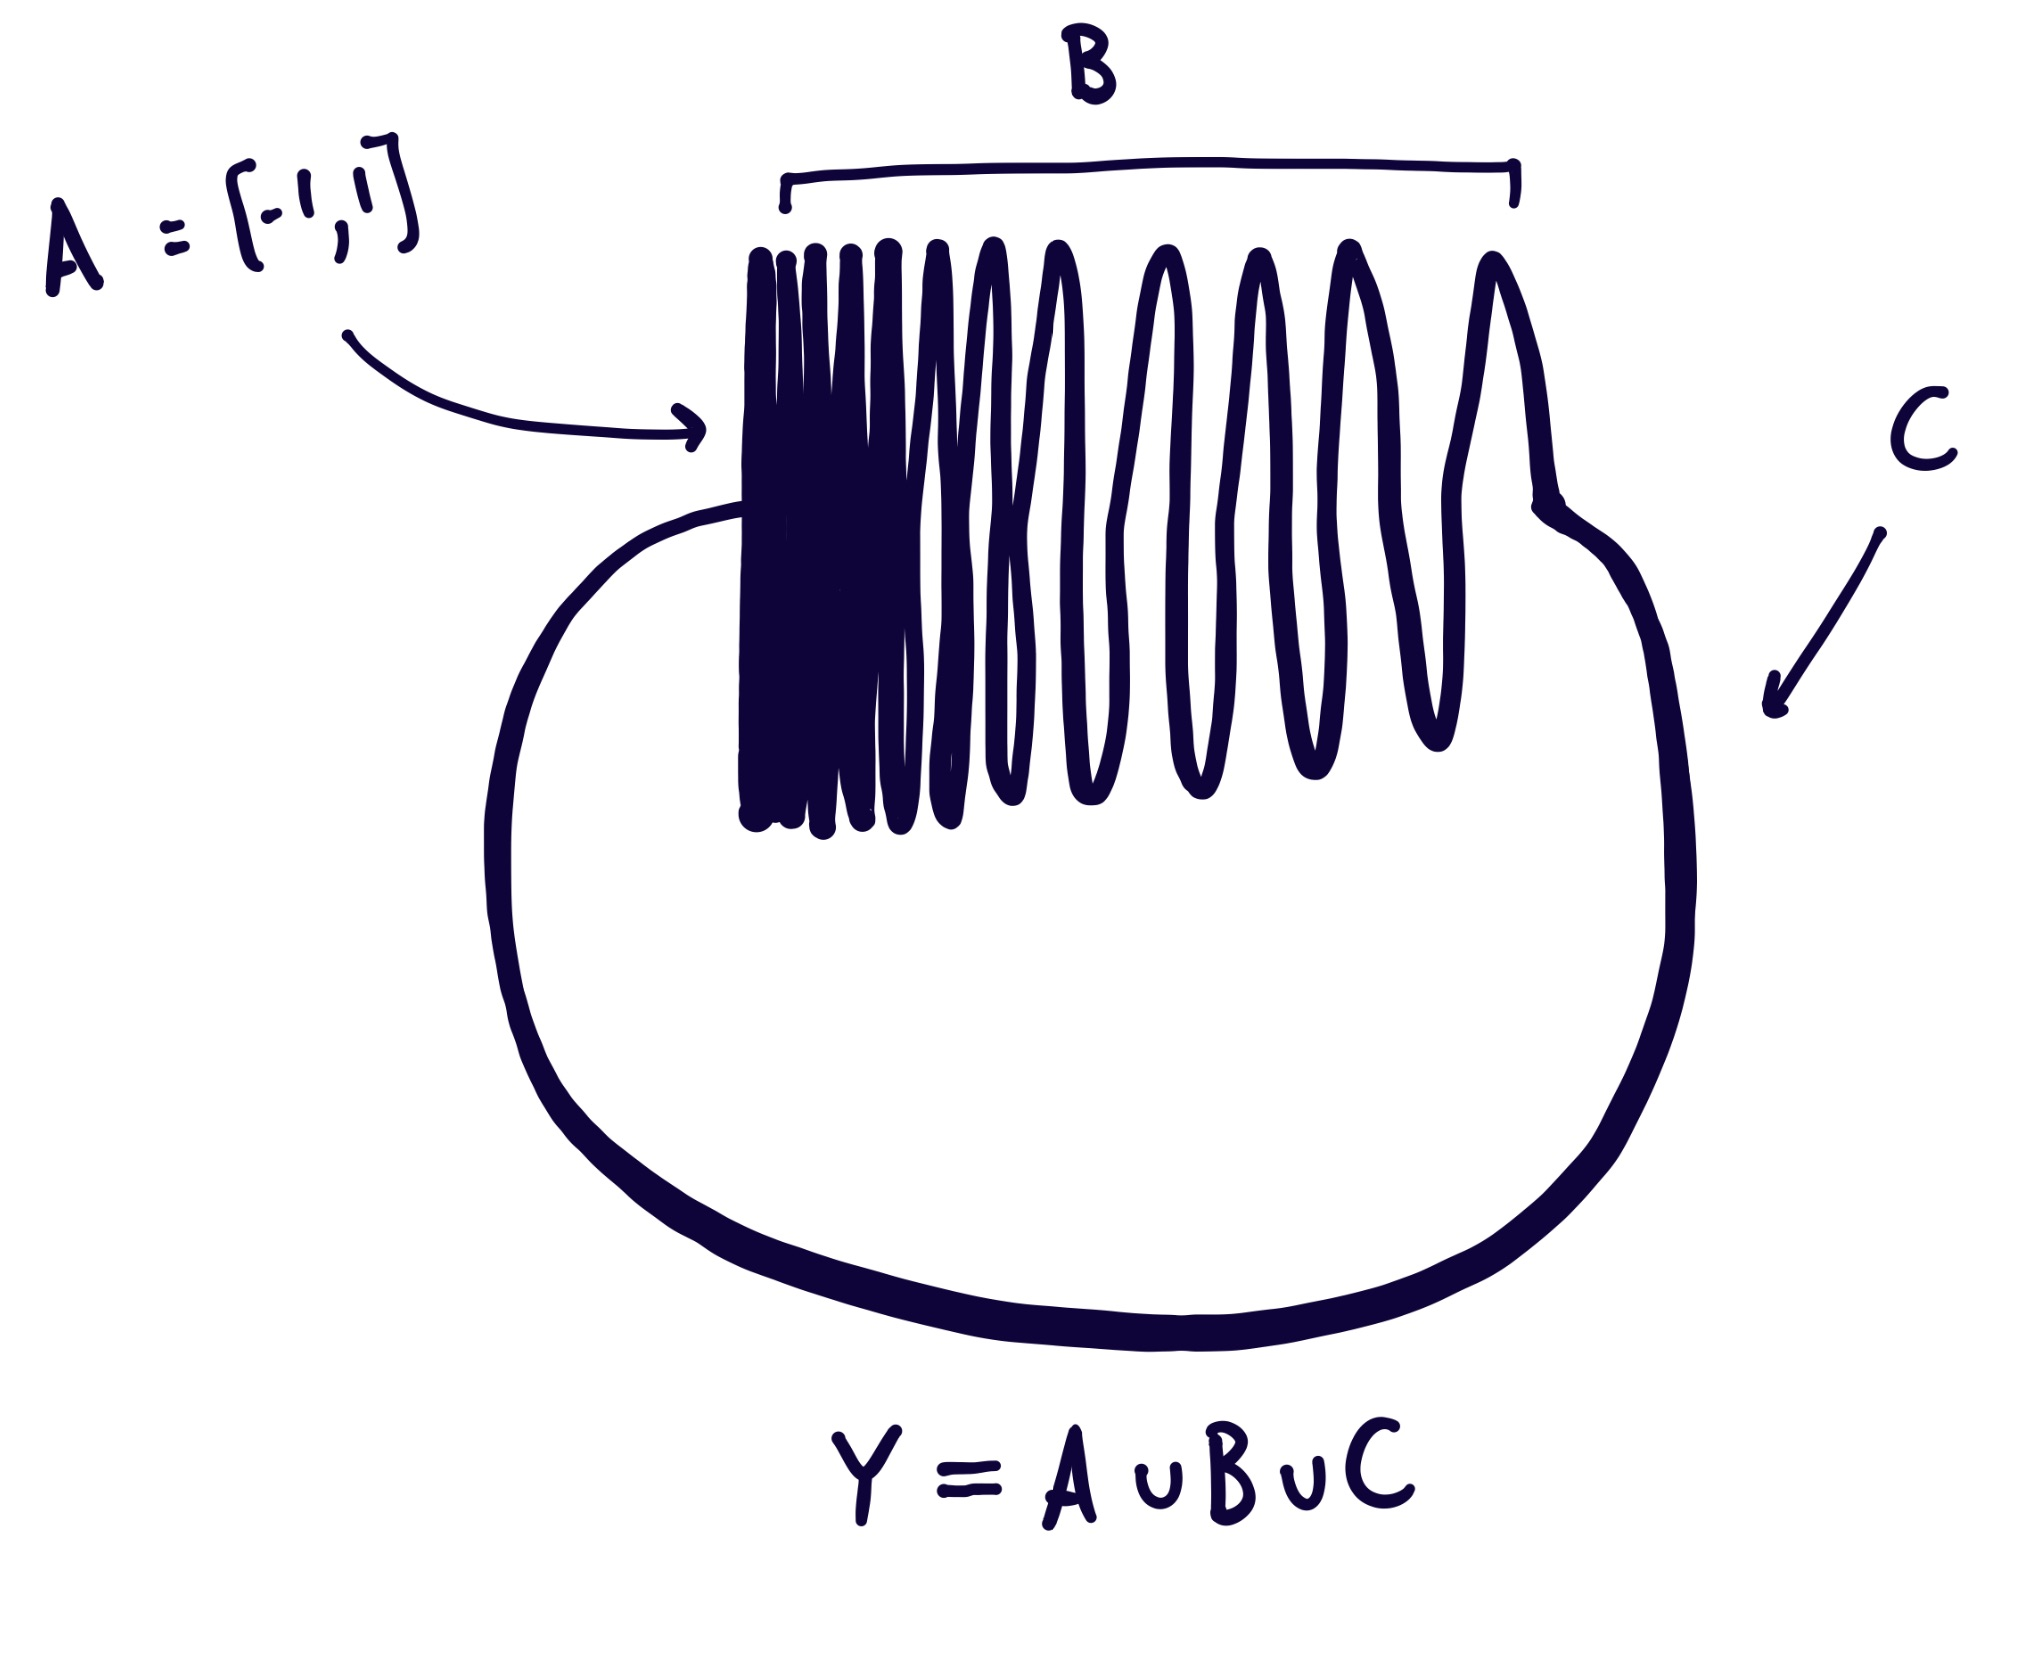
\includegraphics[width=10cm]{figures/hwk6-fig1.jpg}
      \captionof{figure}{The space $Y$ in exercise 1.3.7.} 
      \label{fig:prob1-1}
    \end{center}

    We first argue that $Y$ is path connected. Choose two points $x,y \in Y$. If neither $x$ nor $y$ lies in $A$, then they lie in $B\cup C$, and are hence connected since $B\cup C$ is an embedding of $\bR$. The set $A$ itself is an interval in the $y$-axis and hence connected, and is connected to any point of $B\cup C$ through $(0,0)$. However, $Y$ is not locally path connected. In particular, an open ball around the point $(0,1)$ not containing the origin in $\bR^2$ is not path connected.

    Next we show that $\pi_1(Y,y_0) = 0$, noting that the choice of basepoint does not affect the group due to the path connectedness of $Y$. Consider a loop $\gamma \subseteq Y$. If $\gamma\cap A = \emptyset$, then it is contained in an embedded copy of $\bR$ and is hence nullhomotopic. If $\gamma \cap A \neq \emptyset$, then I claim there is a point $x \in (0,1/2\pi)$ such that $(x,\sin(1/x))\not\in \gamma$. If not, then $\gamma$ would traverse the entirety of the $\sin(1/x)$ curve, which has a limit point at each element of $A$. Such a path would not be the image of a continuous function, and hence would not be a path. Thus, there is a point along $A$ which $\gamma$ does not pass, and we can therefore find a tubular neighborhood of $A$ which does not intersect the portion of $\gamma$ contained in $B$. We can then continuously retract $\gamma \cap A$ to the origin and then into $C$. This proves that every loop in $Y$ is nullhomotopic, and hence $\pi_1(Y) = 0$ as claimed in the problem statement.
    \begin{center}
      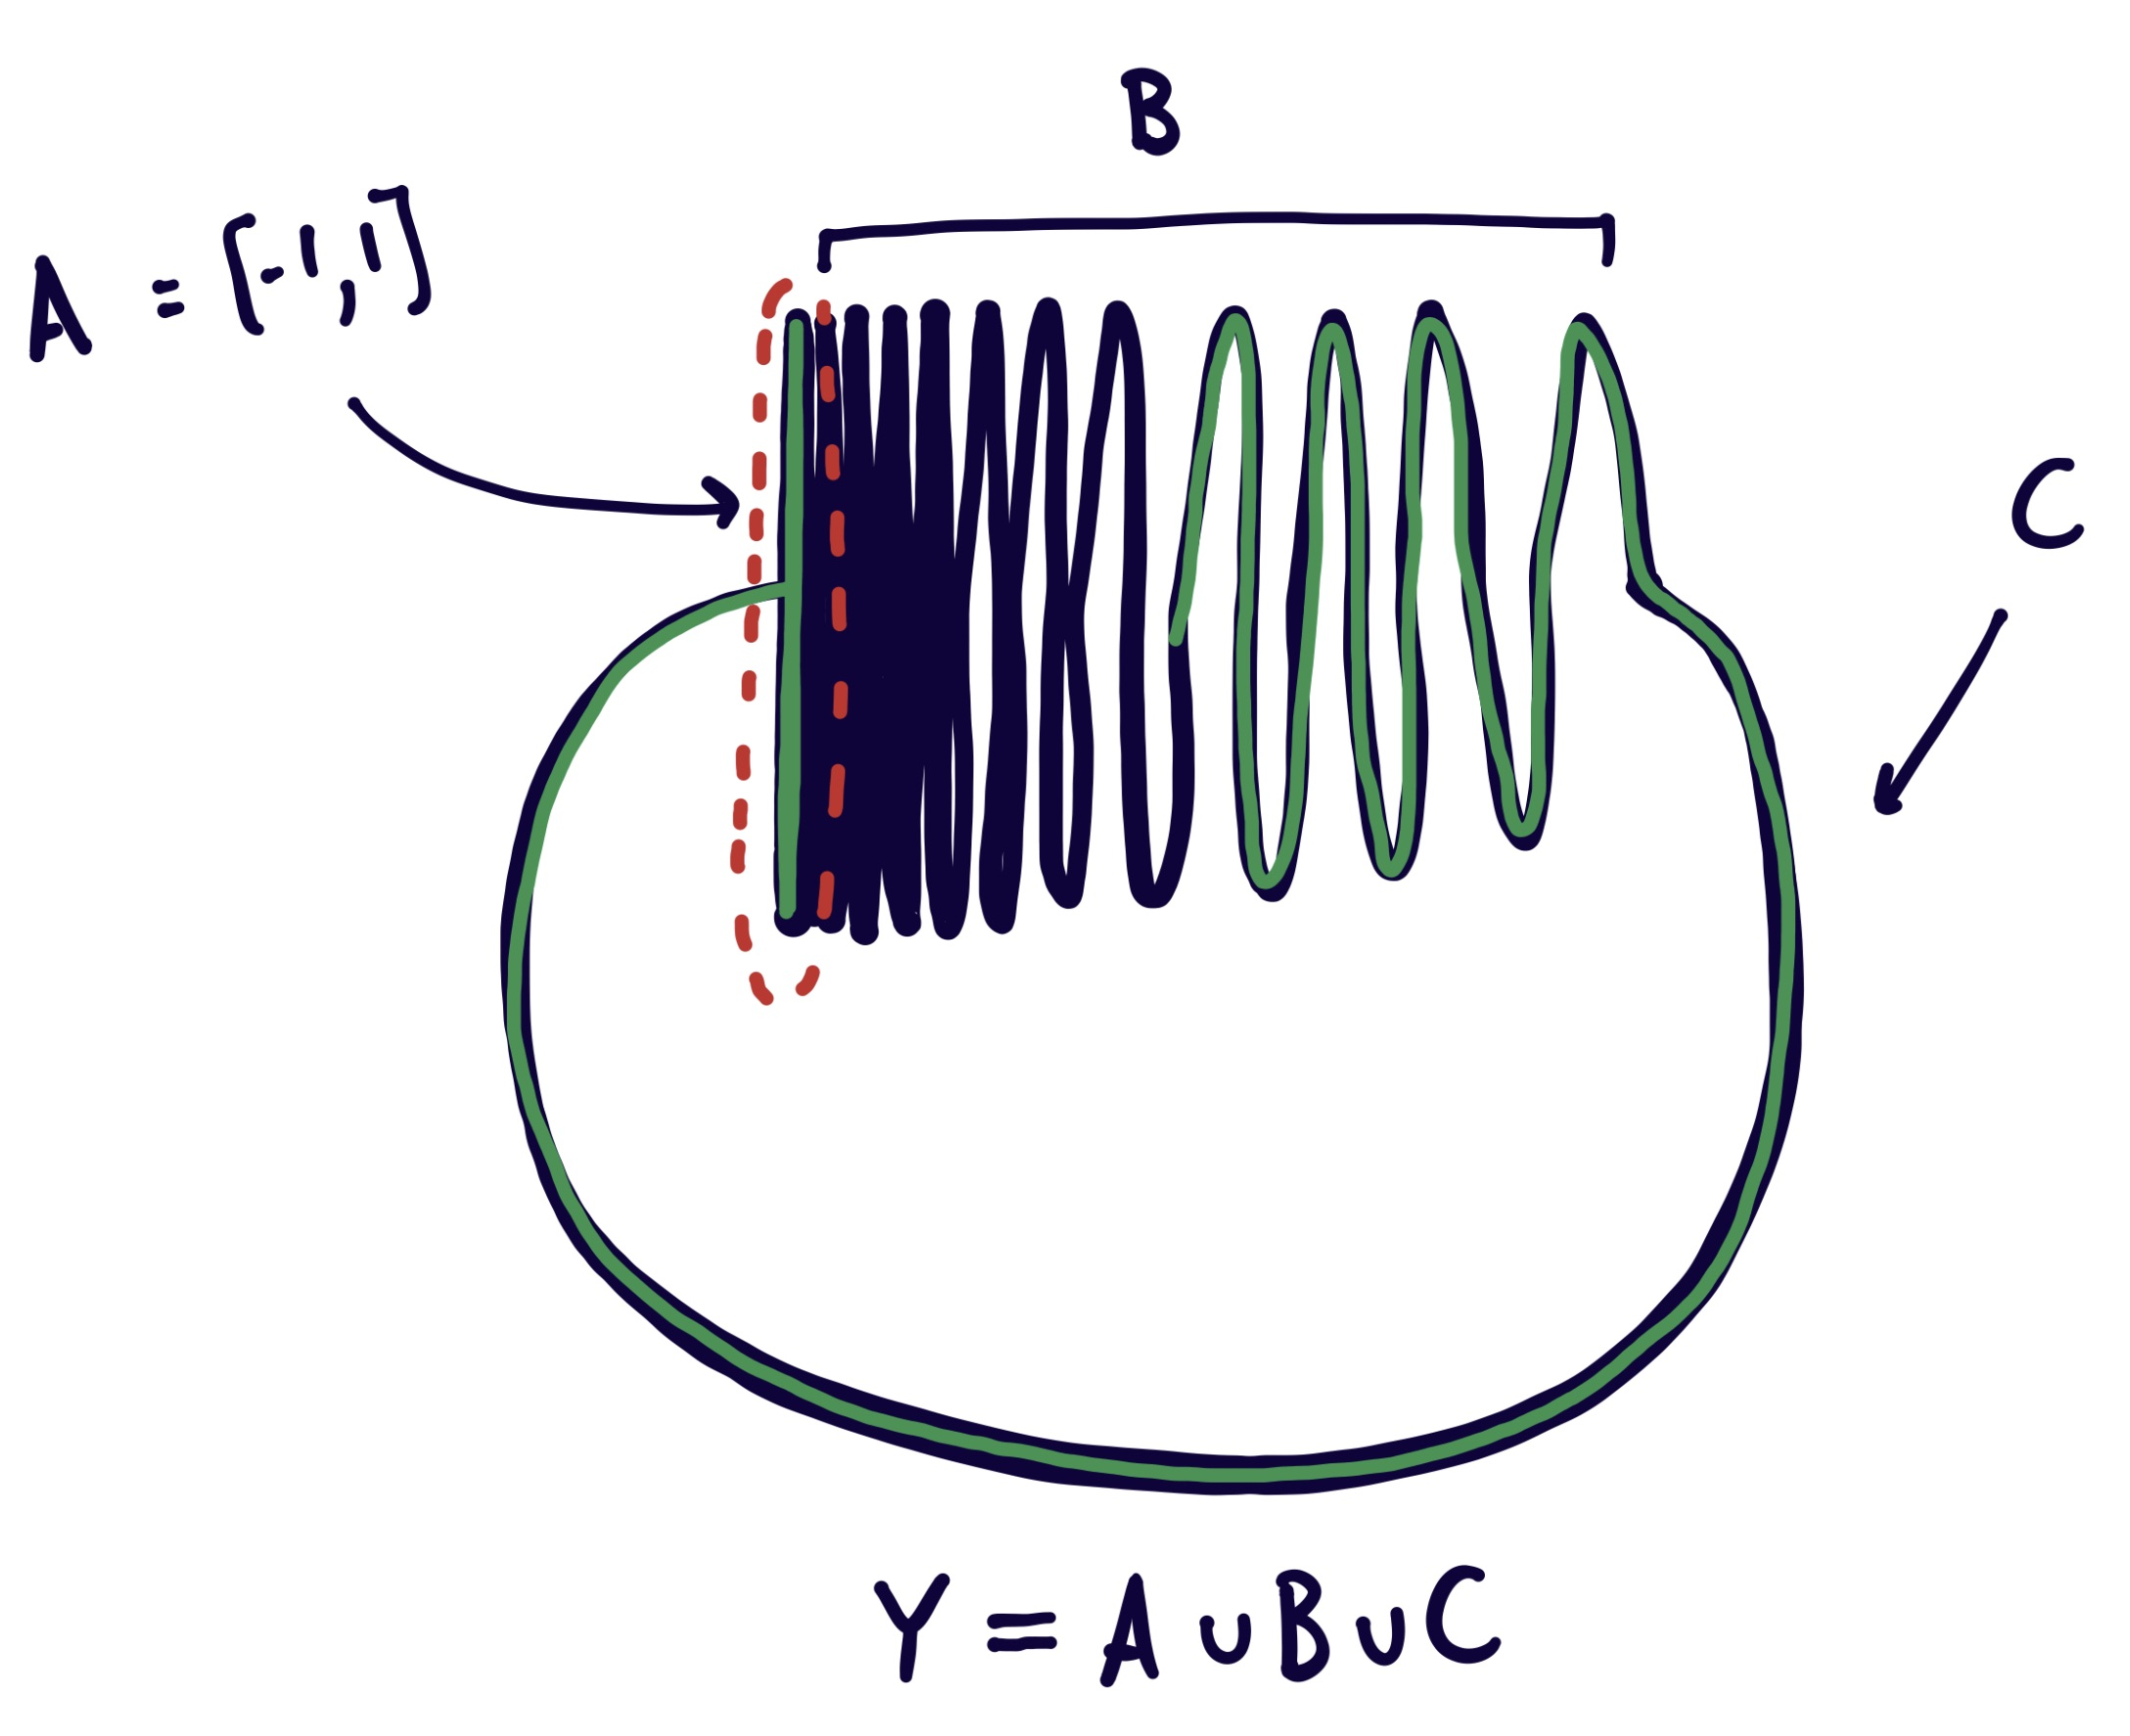
\includegraphics[width=10cm]{figures/hwk6-fig2.png}
      \captionof{figure}{An example of a path $\gamma$ (in green) intersecting $A, B$ and $C$ together with a tubular neighborhood (in red) around $A \cap \gamma$ which does not intersect $\gamma \cap B$.}
      \label{fig:prob1-2}
    \end{center}

    \bigskip

    Let $p:\bR\to S^1$ be the usual covering map, where $S^1$ is realized as the quotient $\bR/\bZ$. Let $s_0$ be the basepoint of $S^1$ achieved by collapsing $A$ to a point, and let $r_0 = 0 \in \bR$ and $y \in Y$ be the basepoints in $\bR$ and $Y$ respectively so that $f(y) = p(r_0) = s_0$. As $f$ is the projection map, it must be the case that $y \in A$.

    Suppose we had a lift $g:Y\to \bR$ so that $p\circ g = f$. Then $g$ must map $B\cup C$ to a component of $p^{-1}(S^1\setminus \{s_0\})$, that is, some open interval $(n,n+1)$. Since $p^{-1}(s_0) = \bZ$, $g(A) \subseteq \bZ$, and then because $g$ must be continuous, it must be constant on $A$. This means $g(Y) = [n,n+1)$ or $(n,n+1]$. Neither of these sets is compact, but $Y$ is -- a contradiction, since the image of a compact set under a continuous function is compact. This shows that local path connectedness is a necessary hypothesis in the lifting criterion.
  \end{prf}

  \prob[\textsc{Exercise 1.3.10}] Find all the connected 2-sheeted and 3-sheeted covering spaces of $S^1 \vee S^1$, up to an isomorphism of covering spaces without basepoints. 

  \begin{prf}
    Let us first find all the connected 2-sheeted covers of $S^1\vee S^1$. Let $s_0\in S^1\vee S^1$ be the basepoint, noting that the choice of basepoint does not affect the fundamental group. Recall that an $n$-sheeted cover lifting a basepoint $x_0$ of a path connected, locally path-connected, semilocally simply-connected space $X$ corresponds to a unique index $n$ subgroup of $\pi_1(X,x_0)$. It therefore suffices to find the index $2$-subgroups of $S^1\vee S^1$ and identify the covers to which they correspond. As every index $2$-subgroup is normal, each index 2 subgroup $N \subseteq \pi_1(S^1\vee S^1,x_0)$ will induce a surjective homomorphism $\varphi:\pi_1(S^1\vee S^1, s_0)\to \bZ_2$, the only group with two elements. Let $\langle a,b \rangle$ be a presentation for $\pi_1(S^1\vee S^1,s_0)$. A homomorphism $\varphi:\pi_1(S^1\vee S^1)\to \bZ_2$ is entirely determined by the images of the generators $a,b$, meaning there are four such homomorphisms only three of which are nontrivial. These are the homomorphisms with their kernels listed:
    \begin{enumerate}[(1)]
      \item $\varphi_1: $ $a \mapsto 1$, $b \mapsto 1$. $~N_1 = \ker \varphi_1 = \langle a^2, ab, b^2 \rangle$
      \item $\varphi_2: $ $a\mapsto 1$, $b\mapsto 0$. $~N_2 = \ker \varphi_2 = \langle a^2,b \rangle$.
      \item $\varphi_2: $ $a\mapsto 0$, $b\mapsto 1$. $~N_3 = \ker \varphi_3 = \langle a,b^2 \rangle$.
    \end{enumerate}
    
    If $p:\tilX \to S^1 \vee S^1$ is a $2$-sheeted covering space of $S^1\vee S^1$, the fiber $p^{-1}(s_0)$ of the basepoint will have two elements. Since $p$ is a local homeomorphism by virtue of being a covering space map, each point $\tilx \in p^{-1}(s_0)$ must locally look like a vertex in a graph with valency 4; or in Hatcher's words, a graph with four ``ends of edges'' at each vertex. This gives us the 3 covering spaces seen in figure. To see that these are the only ones, consider one of the vertices in $\tilX$. If it doesn't have a loop, then it must be connected to the other vertex by two edges, and consequently the other vertex must also have a loop. This corresponds to the subgroups $N_2$ and $N_3$ above. If there is no loop in the graph, then the two vertices must be connected by four edges. There is only one such graph and it corresponds to $N_1$ above. These graphs can be seen in Figure (\ref{fig:prob2-1}).
    \begin{center}
      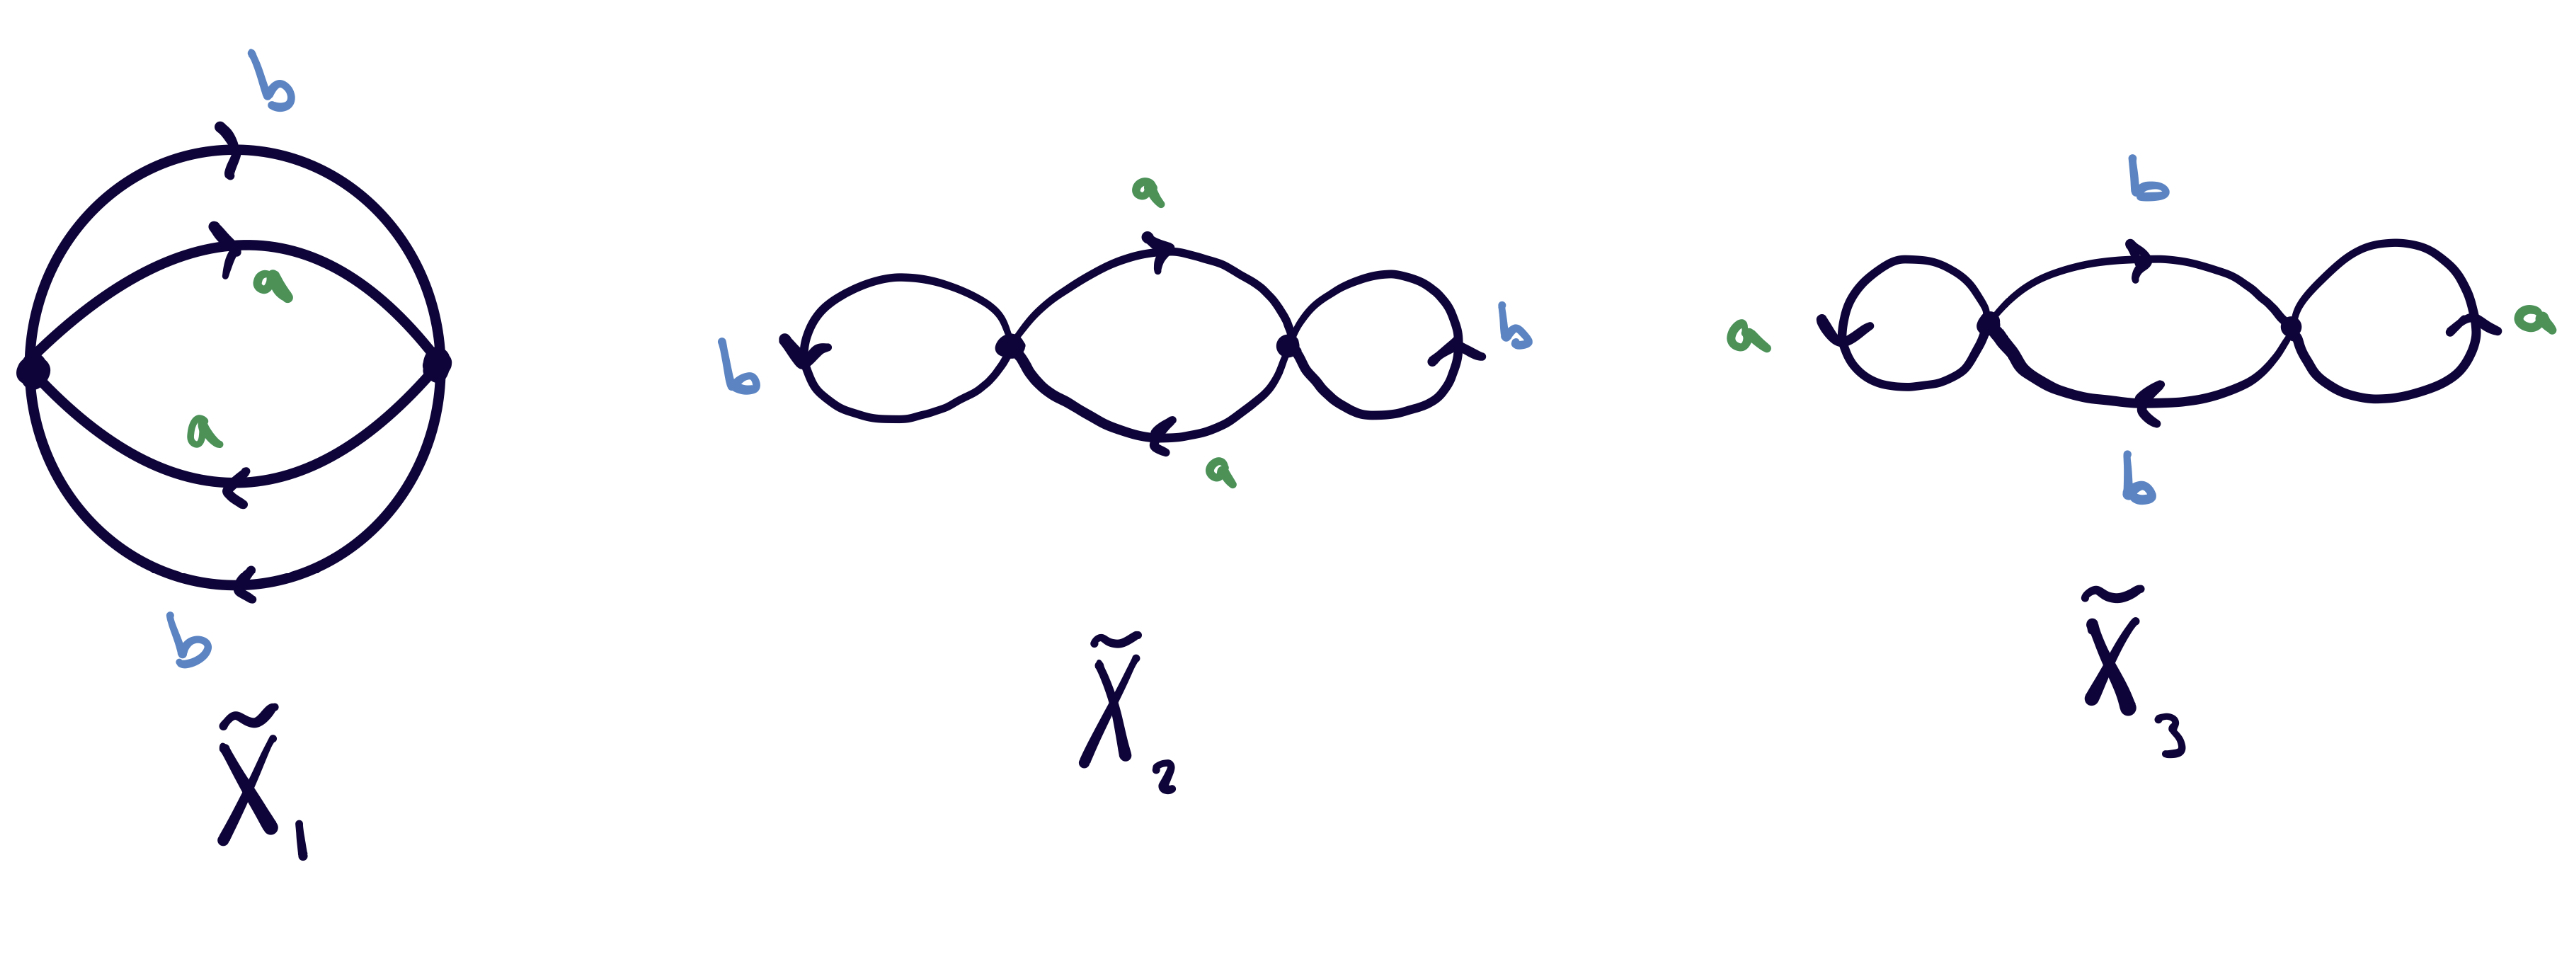
\includegraphics[width=12cm]{figures/hwk6-fig4.jpg}
      \captionof{figure}{The 2-sheeted covers of $S^1\vee S^1$}
      \label{fig:prob2-1}
    \end{center}

    \bigskip

    Now consider the three sheeted covers of $S_1\vee S_1$. These are no longer guaranteed to be normal, so we cannot count them by considering homomorphisms from $F_2$ to order three subgroups. Instead, we carefully consider the possible orientable graphs with three vertices all of valency 4, all of which are seen in Figure (\ref{fig:prob2-2}). We call the vertices $x$, $y$ and $z$ and the basepoint in each graph is denoted with a solid square.

    \textbf{Case 1:} There is a self connection in the graph. Without loss of generality, we may assume it occurs at $x$, i.e. that $x$ has a loop. This leaves $x$ two more ends of edges which must be attached to $x$. It cannot have another loop -- otherwise this graph would not be connected. We then have several subcases.

    \textbf{Case 1.1:} If $x$ is connected to $y$ via two edges, then $y$ is necessarily connected to $z$. Since $y$ must have valency 4, it is hence connected to $z$ twice, and finally $z$ must have a loop. Swapping which edges correspond to $a$ and which correspond to $b$ in this graph does not change the image of its fundamental group in $\pi_1(S^1\vee S^1)$, so we have one isomorphism class of covering space corresponding to $\langle a^2,b^2,aba,bab \rangle$.

    \textbf{Case 1.2:} If $x$ is connected to both $y$ and $z$, then we have three more available connections to $y$ and $z$. Here, we suppose that $y$ also has a loop and treat the other case in Case 1.3. It must then fill its remaining connection with an edge to $z$, which then must also have a loop. By sending the vertices to the wedge point in $S^1\vee S^1$, we see that all the loops are sent to one copy of $S^1$ and all edges between distinct vertices are sent to the other copy. Swapping the labels $a$ and $b$ of the edges then gives us two distinct isomorphism classes of covering spaces which correspond to the subgroups $\langle b,a^3,ababa,aba^2 \rangle$ and $\langle a,b^3,babab,bab^2 \rangle$ in $\pi_1(S^1\vee S^1)$.

    \textbf{Case 1.3:} We now suppose that $x$ has a loop, is connected to both $y$ and $z$ and that $y$ does not have a loop. Since $x$ is already valency 4 under these assumptions, all the remaining connections of $y$ must be made with $z$. This means $y$ and $z$ have three distinct edges between them. Swapping the edge labels gives us two distinct isomorphism classes of coverings spaces corresponding to the subgroups $\langle a,b^3,bab,ba^{-1}b \rangle$ and $\langle b, a^3, aba, ab^{-1}a \rangle$.

    \textbf{Case 2:} If our 3-sheeted cover does \emph{not} contain a self connection, then each pair of vertices necessarily shares 2 connections. Reversing the orientation of the edges gives us two distinct isomorphism classes of covering spaces which correspond to $\langle a^3,b^3,a^{-1}b,ba^{-1} \rangle$ and $\langle a^3, b^3, ab, ba \rangle$.
    
    All together, there are $7$ distinct isomorphism classes of $3$-sheeted covering spaces for $S^1\vee S^1$.

    \begin{center}
      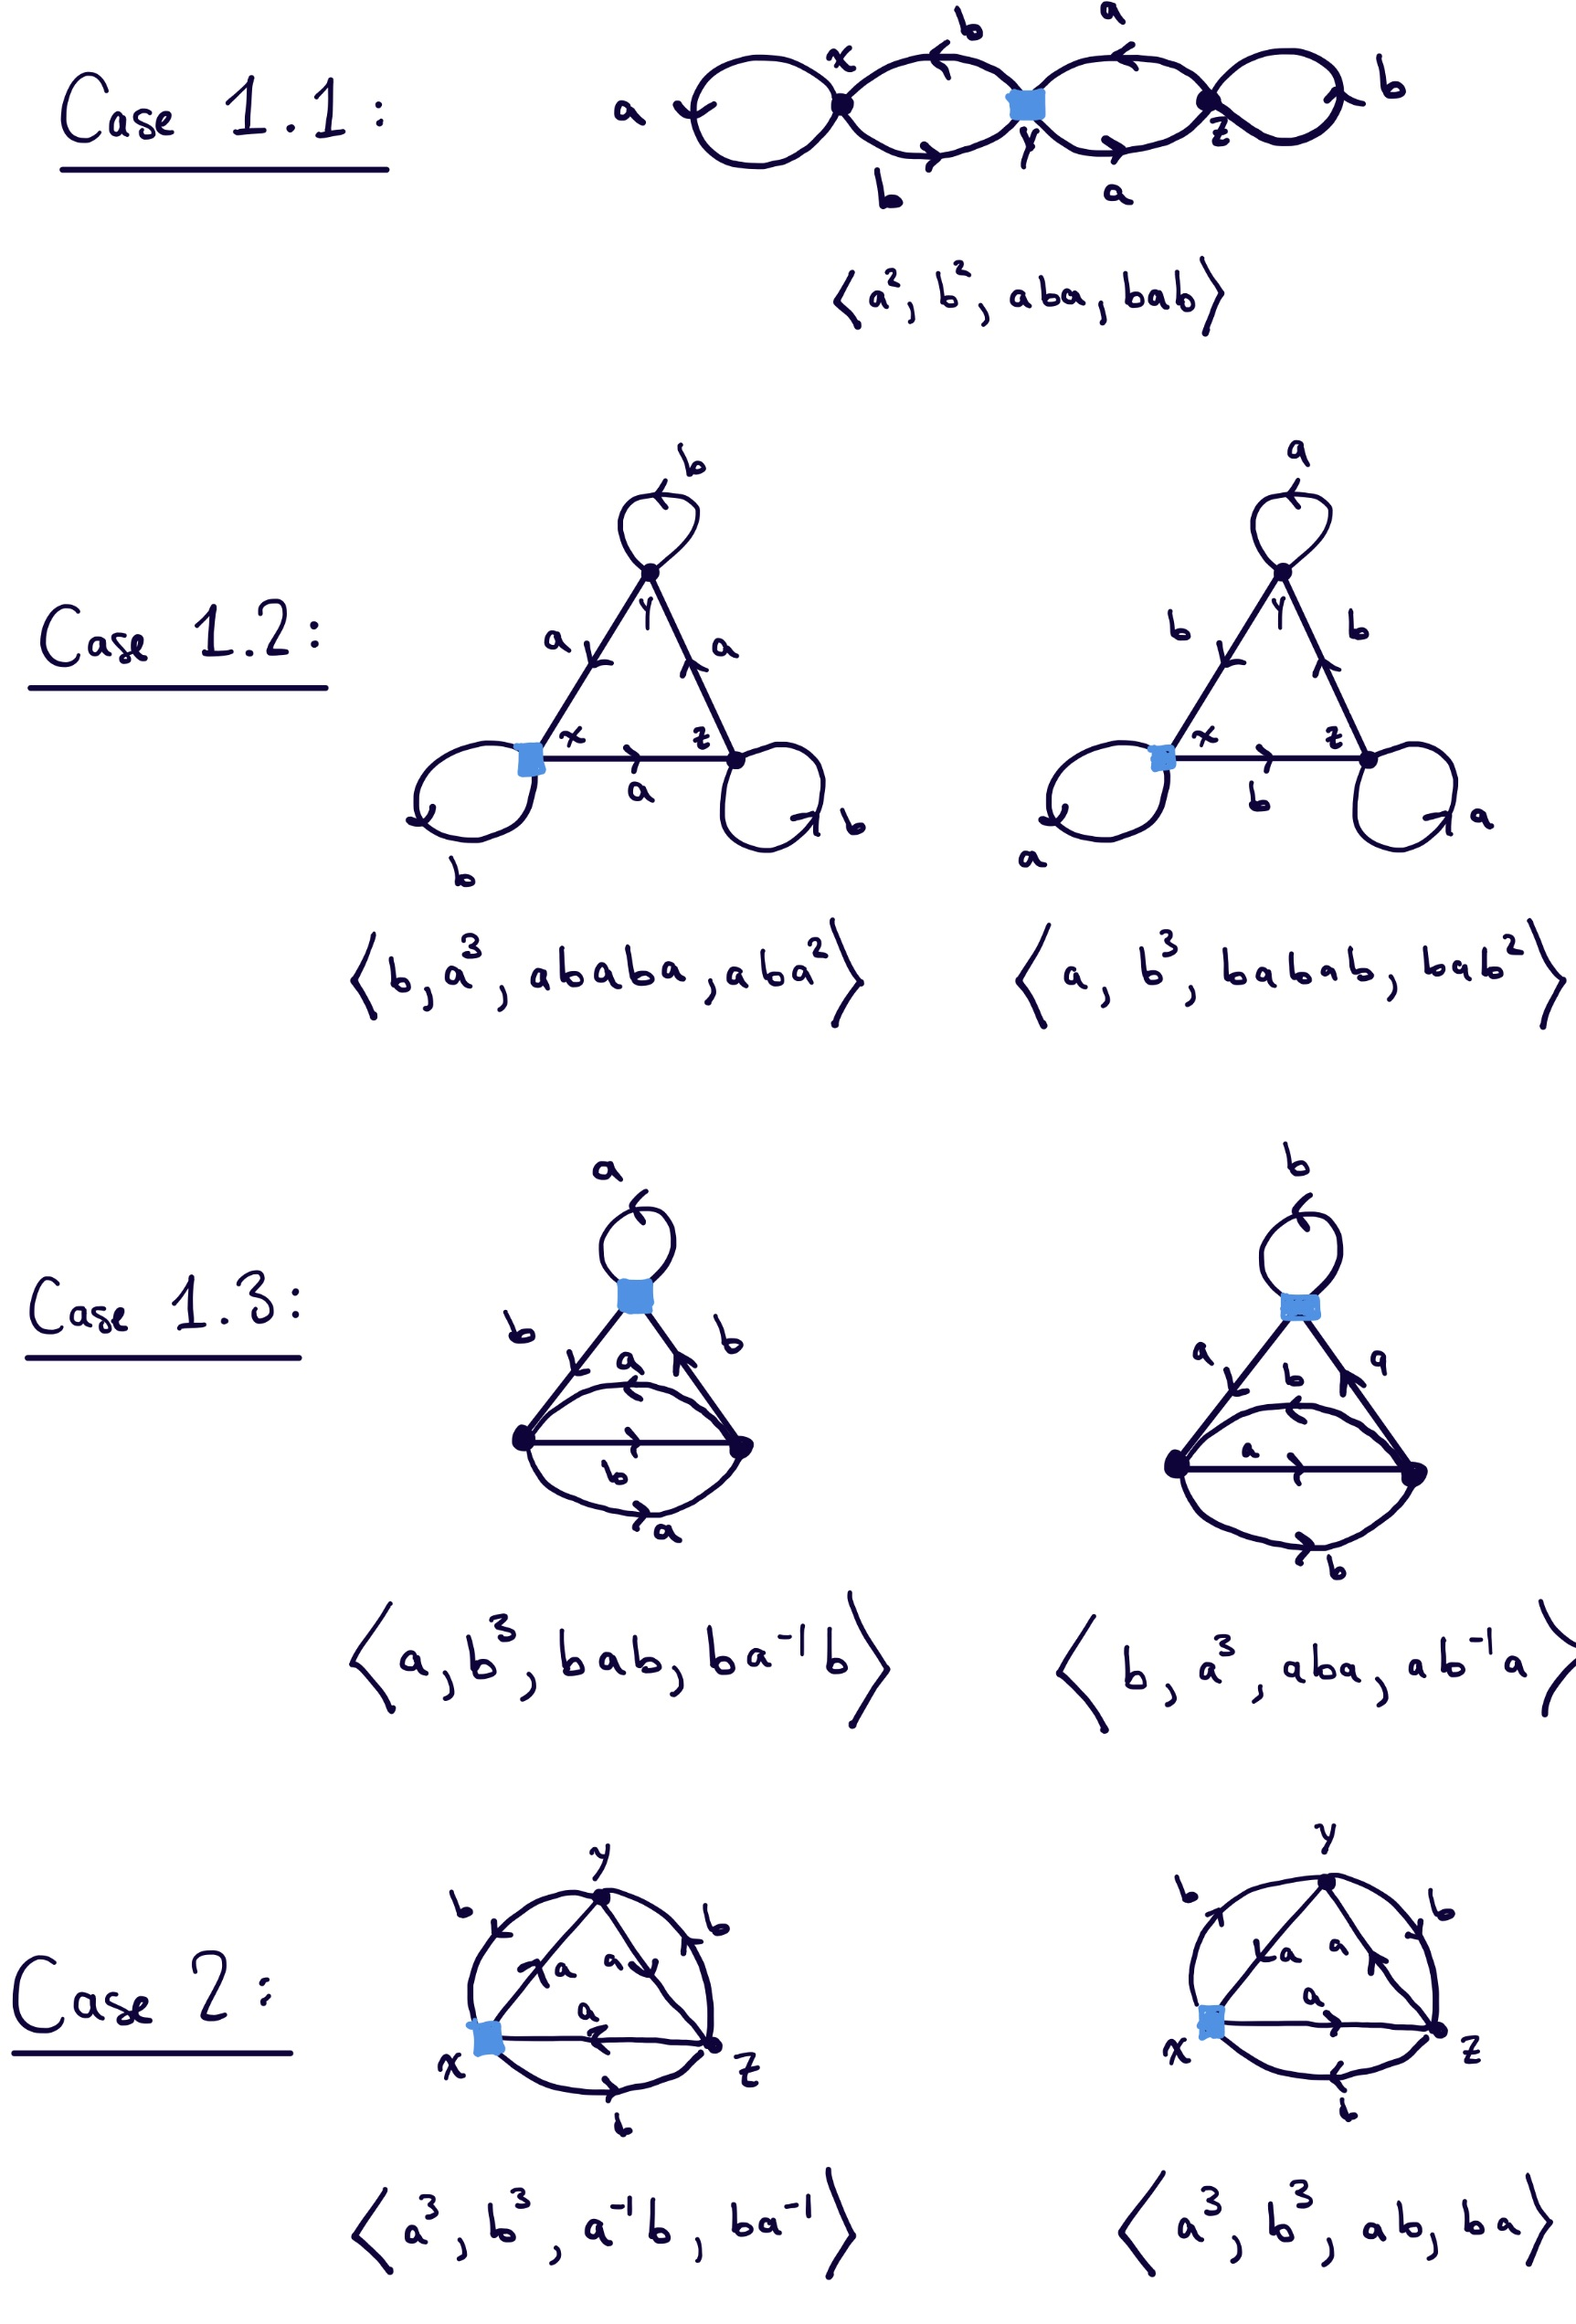
\includegraphics[width=14cm]{figures/hwk6-fig5.png}
      \captionof{figure}{The 3-sheeted covers of $S^1\vee S^1$}
      \label{fig:prob2-2}
    \end{center}

  \end{prf}
  \prob[\textsc{Exercise 1.3.11}] Construct finite graphs $X_1$ and $X_2$ having a common finite-sheeted covering space $\tilX_1 = \tilX_2$ but such that there is no space having both $X_1$ and $X_2$ as covering spaces.
  \begin{prf}
    Figure (\ref{fig:prob3-1}) comprises the primary content of this solution. Let $X_1$ be the connected graph with two vertices, each with a single self-connection, and let $X_2$ be the graph with two vertices with three edges between them. 

    I claim that neither of these graphs is a covering space for any space besides themselves. Indeed, any space $X$ which admitted either $X_1$ or $X_2$ as a cover would necessarily be a graph with either $1$ or $2$vertices. If $X$ had two vertices, then the covering map would simply be the identity. If $X$ had one vertex, then it's valency would necessarily match the valency of the vertices in $X_1$ and $X_2$, all of which are valency $3$. However, the sum of valencies of a finite graph is equal to twice the number of edges, and in particular, is even.

    Nonetheless, $X_1$ admits the cover $\tilX_1$ and $X_2$ admits the cover $\tilX_2$, both of which are described in Figure (\ref{fig:prob3-1}). As topological spaces, $\tilX_1 \cong \tilX_2$.

    \begin{center}
      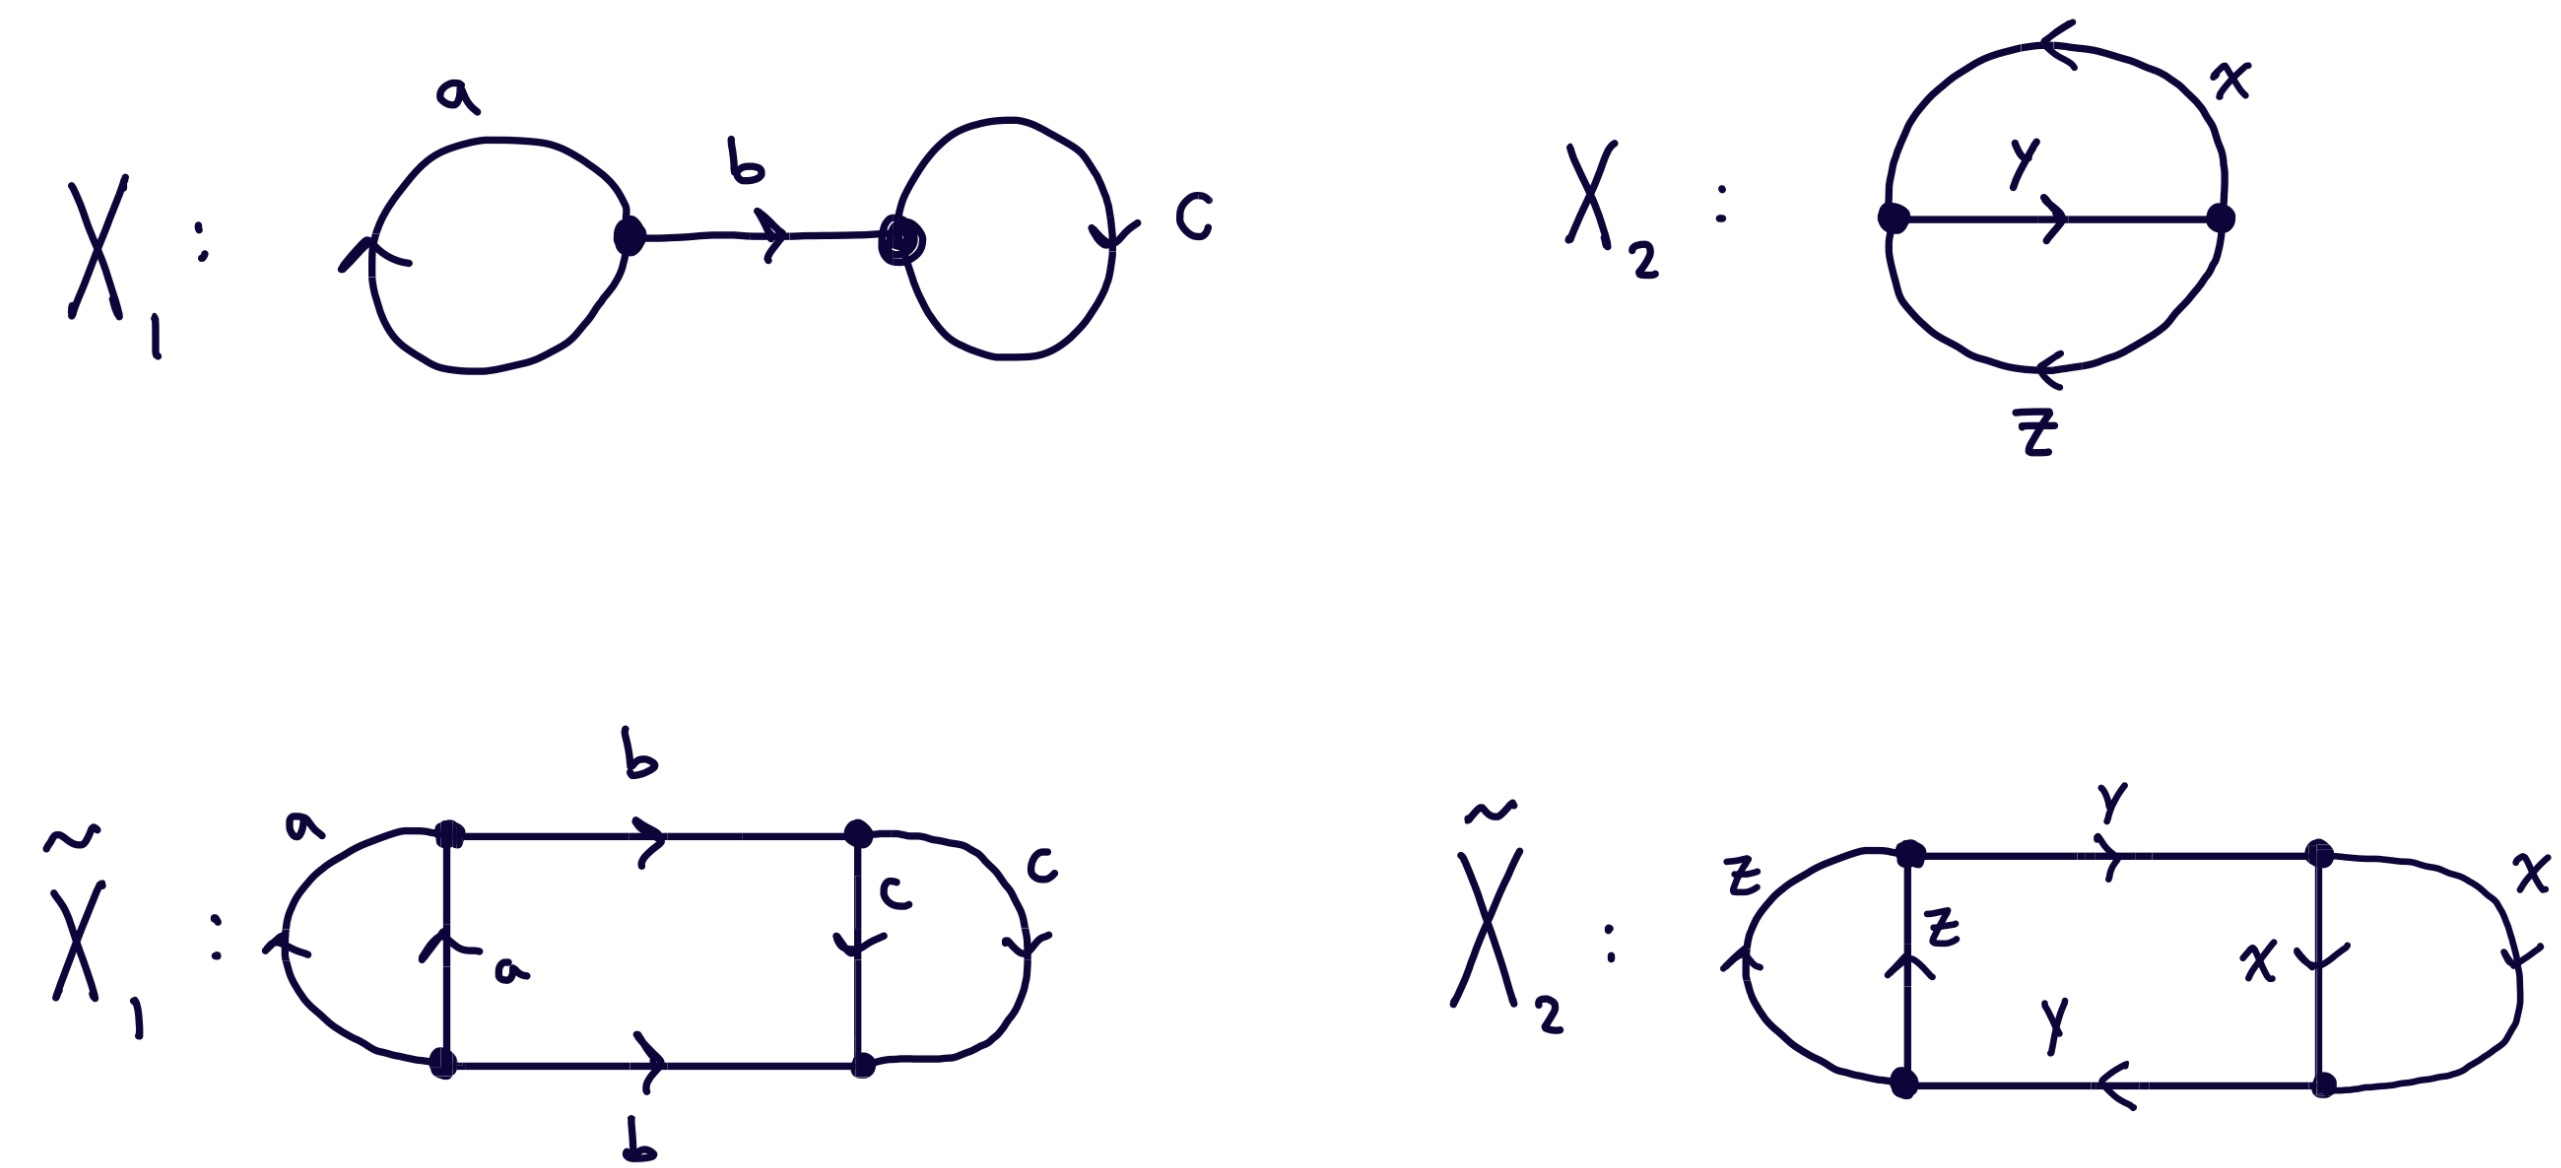
\includegraphics[width=15cm]{figures/hwk6-fig3.png}
      \captionof{figure}{Two graphs $X_1$ and $X_2$ which admit isomorphic coverings spaces but which are not themselves not both covers of another space.} 
      \label{fig:prob3-1}
    \end{center}
  \end{prf}
  \prob[\textsc{Exercise 1.3.18}] For a path-connected, locally path-connected, and semilocally simply-connected space \emph{X}, call a path connected covering space $\overset{\sim}{X}$ \emph{Abelian} if it is normal and has Abelian deck transformation group. Show that $X$ has an Abelian covering space that is a covering space of every other Abelian covering space of $X$, and that such a universal Abelian covering space is unique up to isomorphism. Describe this covering space explicitly for $X = S^1 \vee S^1$ and $X = S^1 \vee S^1 \vee S^1$.
  \begin{prf}
    Our space $X$ has a universal cover $\tilX$. By Proposition 1.39 in Hatcher, every normal cover of $X$ has the form $Y = \tilX / H$, where $H$ is a normal subgroup of $G = \pi_1(X,x)$. In such a case, the Deck Transformation group $\Aut(Y/X) \cong G/H$, hence $Y$ is an Abelian cover if and only if $H$ is normal in $G$ and $G/H$ is Abelian. It is a general fact from group theory that $G/H$ is Abelian if and only if $H$ contains the commutator subgroup $G_0 = [G,G]$ of $G$. By the covering space correspondence theorem, there is a (necessarily Abelian) covering space $\tilX^{ab}$ of $X$ associated to the commutator subgroup $G_0$. By our discussion above, a covering space $Y$ of $X$ is normal if and only if its associated subgroup $\pi_1(Y,y) \cong H \subseteq G$ is normal and Abelian. Since $G_0$ is contained in $H$, $\tilX$ is a covering space of $Y$, again by the correspondence theorem. Hence $\tilX$ is a universal Abelian cover in the sense described by the problem statement.

    Suppose now that we had some other universal Abelian covering space $Y$ of $X$ with covering map $p_*:Y\to X$. Then the subgroup $H = p_*(\pi_1(Y,y))$ of $G = \pi_1(X,x)$ associated to $Y$ is normal and $G/H$ is Abelian. This implies that $G_0 \subseteq H$, again by basic group theory. However, since $Y$ was assumed to be a universal Abelian cover, we have a covering map $q:Y \to \tilX^{ab}$, and hence $q_*(\pi_1(Y,y))\subseteq \pi_1(\tilX^{ab},\tilx)$ by the correspondence theorem. Since the map induced by covering maps on fundamental groups is always injective, we have isomorphisms $G_0 \cong \pi_1(\tilX^{ab},\tilx)$ and $q_*(\pi_1(Y,y))\cong \pi_1(Y,y) \cong H$, meaning we have an inclusion $H \subseteq G_0$. This means $H = G_0$, so $Y$ and $\tilX^{ab}$ are isomorphic as covering spaces over $X$.

    \bigskip

    Now set $X = S^1\vee S^1$. The universal Abelian cover $\tilX^{ab}$ of $X$ corresponds to the commutator subgroup of $\pi_1(X) \cong \bZ\ast \bZ$, which is $\bZ\times \bZ$. Since the universal Abelian cover is unique up to isomorphism, we simply need to find a space whose fundamental group is $\bZ\times \bZ$. The infinite lattice $\bZ\times \bZ \subseteq \bR^2$ together with the line segments connecting nearest neighbor points is one such space. As a set, it is
    \begin{align*}
      \tilX^{ab} = \left\{(x,y) \in \bR^2 \midd x \in \bZ ~\text{ or }~ y\in \bZ\right\}.
    \end{align*}

    A nearly identical argument gives us the universal Abelian cover for $\tilX^{ab}$, which is 
    \begin{align*}
      \tilX^{ab} = \left\{(x,y,z) \in \bR^3 \midd (x,y) \in \bZ^2 ~\text{ or }~ (x,z) \in \bZ^2 ~\text{ or }~ (y,z)\in \bZ^2\right\}.
    \end{align*}
  \end{prf}

  \prob[\textsc{Exercise 1.3.19}] Use the preceding problem to show that a closed orientable surface $M_g$ of genus $g$ has a connected normal covering space with deck transformation group isomorphic to $\bZ^n$ (the product of $n$ copies of $\bZ$) if and only if $n \leq 2g$. For $n = 3$ and $g \geq 3$, describe such a covering space explicitly as a subspace of $\bR_{63}$ with translations of $\bR^3$ as deck transformations.
  \begin{prf}
    First, recall that the fundamental group of $M_g$ is
    \begin{align*}
      \pi_1(M_g) = \langle a_1,b_1,...,a_g,b_g ~\mid~ [a_1,b_1]\cdot...\cdot[a_g,b_g] = 1 \rangle.
    \end{align*}
    The Abelianization of this group is the free Abelian group on $2g$ generators, i.e. $\bZ^{2g}$. As in problem 1.3.18 above, let $G_0$ denote the commutator subgroup of $\pi_1(M_g)$, so that $\pi_1(M_g)/G_0 \cong \bZ^{2g}$.

    Suppose now that $Y$ is a normal covering space with associated subgroup $H$ of $\pi_1(M_g)$ and whose deck transformation group isomorphic to $\bZ^n$. Since $Y$ has Abelian deck transformation group, $H$ must contain $G_0$ by the results of problem 1.3.18. By theorem 1.39 (which gives us an isomorphism between deck transformation groups for normal covers and the quotient group given by their associated subgroup) and the third isomorphism theorem, we have
    \begin{align*}
      \bZ^n \cong \pi_1(M_g)/H \cong (G/G_0)/(H/G_0) \cong \bZ^{2g}/(H/G_0).
    \end{align*}
    Since any free group obtained as a quotient of $\bZ^{2g}$ has rank at most equal to $2g$, we have $n \leq 2g$.

    \bigskip

    Now consider the case of $M_3$. We wish to describe the covering space whose deck transformation group is $\bZ^3$. This covering space will be a surface in $\bR^3$ invariant under the action of $\bZ^3$, which acts by translation. This covering space will morally be comprised of tubular neighborhoods of integer translations of the interval $[1/4,3/4]$ around each coordinate axes in $\bR^3$ together with copies of $S^2$ with six disks removed connecting them. An attempt at drawing the fundamental domain of the $\bZ^3$ action on this covering space can be viewed in Figure (\ref{fig:prob5-1}).
    \begin{center}
      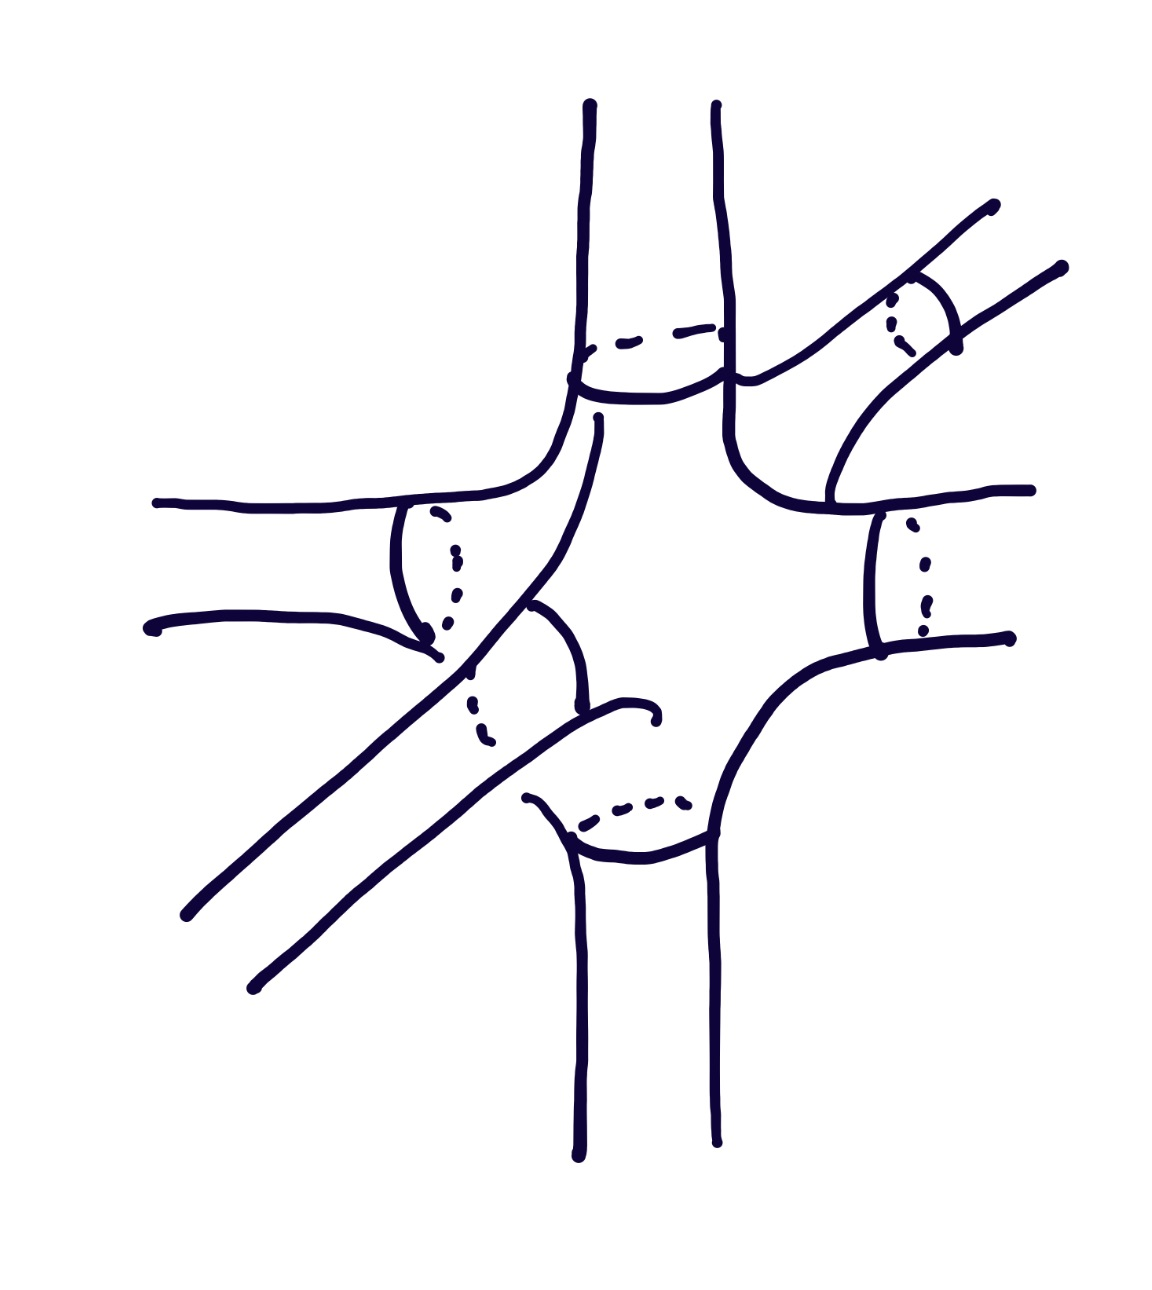
\includegraphics[width=8cm]{figures/hwk6-fig6.png}
      \captionof{figure}{Fundamental domain of the covering space of $M_g$ corresponding under the action of $\bZ^3$, its deck transformation group.} 
      \label{fig:prob5-1}
    \end{center}

    An easier way to construct this space is to realize the we only need the spheres. Let $S$ be the sphere $S^2$ of radius $5/4$ centered at the origin in $\bR^3$. Remove from $S$ all points not contained in the box $[-1,1]^3\subseteq \bR^3$ centered at the origin and call this new set $\Gamma$. This is equivalent to removing six disjoint disks from the surface of $S$. The set $\Gamma$ is pictured in figure (\ref{fig:prob5-2}).
    \begin{center}
      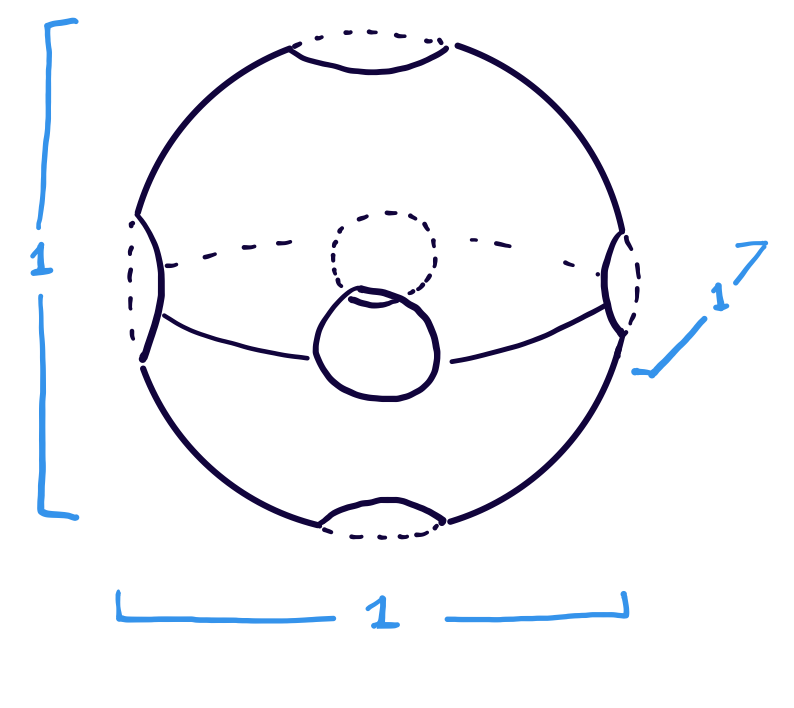
\includegraphics[width=10cm]{figures/hwk6-fig7.png}
      \captionof{figure}{The set $\Gamma$ obtained by removing six disks from the sphere $S$.} 
      \label{fig:prob5-2}
    \end{center}

    Now take the image of $\Gamma$ under the action of $\bZ^3$. This yields a surface consisting of copies of $\Gamma$ at every $\bZ$-point in $\bR^3$ connected by the boundaries of the deleted disks. A portion of this space is pictured in Figure (\ref{fig:prob5-3}).
    \begin{center}
      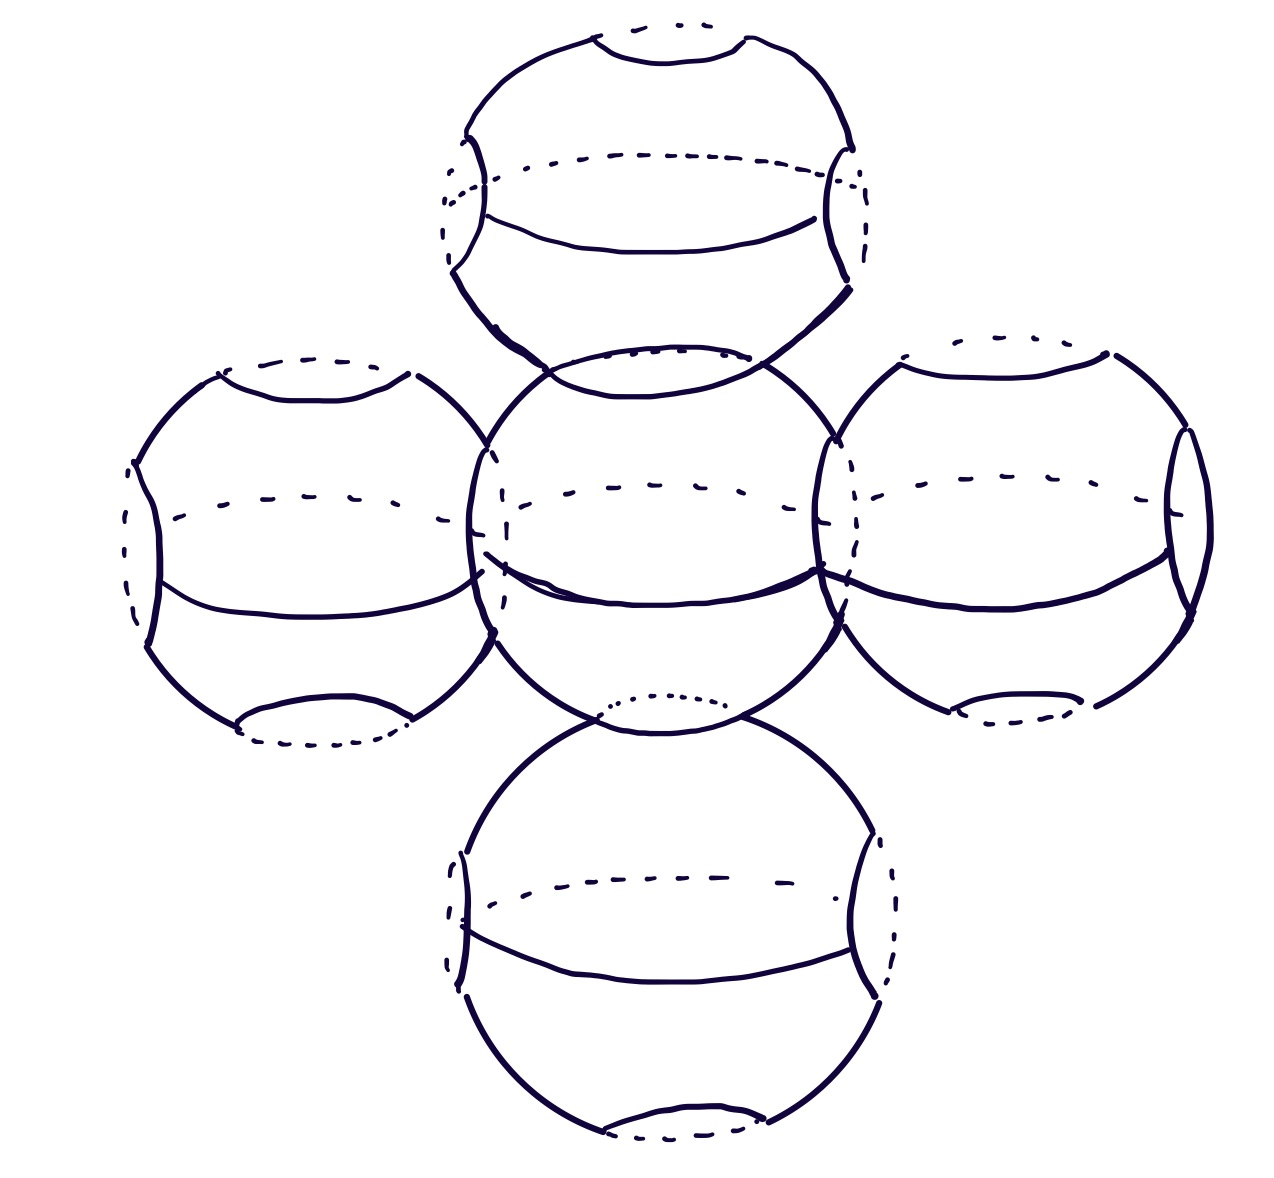
\includegraphics[width=12cm]{figures/hwk6-fig7.jpg}
      \captionof{figure}{Alternative, easier-to-draw-and-define portion of covering space of $M_g$.} 
      \label{fig:prob5-3}
    \end{center}
    This is the covering space of $M_g$ whose deck transformation group is $\bZ^3$.
  \end{prf}
\end{homework}
\end{document}
